\documentclass[a4paper,12pt]{article}
\usepackage[utf8]{inputenc}      % Codificación UTF-8 para caracteres en español
\usepackage[T1]{fontenc}         % Buena salida de fuentes
\usepackage[spanish]{babel}      % Traducción de elementos automáticos al español
\usepackage{lmodern}             % Fuente mejorada
\usepackage[hidelinks]{hyperref} % Para enlaces, [hidelinks] elimina el reborde azul del .pdf
\usepackage{graphicx}            % Para incluir imágenes (PNG)
\usepackage{float}               % Para anclar las imagenes a una posicion fija
\usepackage{bytefield}           % Para dibujar diagramas PDU
\usepackage{geometry}            % Para ajustar márgenes
\geometry{left=2.5cm, right=2.5cm, top=3cm, bottom=3cm}

\title{El protocolo IPv6}
\author{Martín Moloeznik, Nicolás Paz Reyes\\[0.5em]
Repositorio: \url{https://github.com/tu_usuario/tu_repositorio}}
\date{\today}

\begin{document}

% Carátula
\begin{titlepage}
  \centering
  \vspace*{2cm}
  {\large \textbf{El protocolo IPv6}}\\[1.5cm]
  
  {\large Integrantes:}\\
   \bigskip
  {\large Martín Moloeznik, Nicolás Paz Reyes} \\[0.5cm]
  {\large {martinmoloeznik@gmail.com}, {rubenpaz2105@gmail.com}} \\[0.5cm]
  \bigskip
  {\large Repositorio: \url{https://github.com/N1C0-P4Z/Protocolo-IPv6}}\\[1cm]
  
  \vfill
  {\large \today}
\end{titlepage}

% Índice (opcional)
\tableofcontents
\newpage

% Sección de Introducción
\section{Introducción}
El protocolo IPv6 fue desarrollado para reemplazar a IPv4 debido a la necesidad de una mayor cantidad de direcciones IP en el mundo. Dentro de IPv6 existen mecanismos esenciales para la configuración de direcciones y la comunicación entre dispositivos, entre los cuales se destacan SLAAC, EUI-64 y el protocolo Neighbor Discovery (NDP).

% Sección 1: Escenarios y Configuraciones
\section{IPv6 SLAAC and EUI-64 Basics}
\subsection{Configuración del Router en IPv6}
\begin{figure}[H]
  \centering
  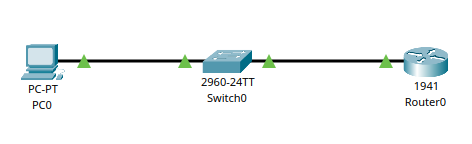
\includegraphics[width=0.7\textwidth]{imagenes/lab1.png}
  \caption{Red a ensayar}
  \label{fig:lab1}
\end{figure}

Mediante los siguientes comandos configuramos la Link Local Address del router a fe80::1 y la GUA a 2001:db8:acad:1::1/64.\\

\noindent Router\#enable\\
Router\#configure terminal\\
Router(config)\#ipv6 unicast-routing\\
Router(config)\#interface g0/0\\
Router(config-if)\#ipv6 enable\\
Router(config-if)\#ipv6 address fe80::1 link-local\\
Router(config-if)\#ipv6 address 2001:db8:acad:1::1/64\\
Router(config-if)\#no shutdown\\

\subsection{Explicacion algoritmo EUI-64}
   La pc se autoconfigura su Link Local Addres siguiendo los pasos a continuacion:

\bigskip
\begin{bytefield}[boxformatting={\centering\itshape},bitwidth = 1.1em]{32}
  \begin{rightwordgroup}{Algoritmo \\ EUI-64}

    \bitbox{16}{48 bit MAC} & \bitbox{16}{00-E0-F9-98-8A-07}\\
    \bitbox{16}{Separa al medio} & \bitbox{16}{00-E0-F9 \hspace{0.45cm} | \hspace{0.45cm} 98-8A-07}\\
    \bitbox{16}{Insertar FF-FE} & \bitbox{16}{00-E0-F9 \textbf{FF-FE} 98-8A-07}\\
    \bitbox{16}{Primeros dos hexa a binario} & \bitbox{16}{0000-0000-E0-F9  \textbf{FF-FE} 98-8A-07}\\
    \bitbox{16}{Se invierte el septimo bit} & \bitbox{16}{0000-00\textbf{1}0-E0-F9  \textbf{FF-FE} 98-8A-07}\\
    \bitbox{16}{64 bits host interface ID} & \bitbox{16}{\textbf{02}-E0-F9-\textbf{FF-FE}-98-8A-07}\\
    \bitbox{16}{Link Local Address} & \bitbox{16}{FE80::\textbf{2E0:F9FF:FE98:8A07}}
  \end{rightwordgroup}
\end{bytefield}

\bigskip
\texttt{Luego entramos al modo simulación y cambiamos la configuración ipv6 de la pc de static a  auto-config, inmediatamente, la pc envía un mensaje de router solicitation. Donde la ip de origen es la LLA de la pc que se autoconfiguró mediante EUI-64 y la ip destino es la ALL routers multicast address.}
\bigskip

\begin{bytefield}[boxformatting={\centering\itshape},bitwidth = 1.1em]{32}
  \bitheader{0,4,12,32} \\
  \bitbox{4}{Ver:6} & \bitbox{8}{TRFC} & \bitbox{20}{FLOW LABEL}\\
  \bitbox{16}{PL:12} & \bitbox{8}{NEXT:0x3a} & \bitbox{8}{HOP LIMIT:255}\\ 
  \begin{rightwordgroup}{Link Local\\ Address}
    \wordbox{2}{SRC IP:FE80::2E0:F9FF:FE98:8A07}
  \end{rightwordgroup}\\
  \begin{rightwordgroup}{All Routers\\ Multicast \\address}
    \wordbox{2}{DEST IP:FF02::2}
  \end{rightwordgroup}
\end{bytefield}

\texttt{La PC aprende que se esta usando IPv6 y a la LLA del router que usará como gateway.}

\section*{IPv6 Packet}
\begin{bytefield}[boxformatting={\centering\itshape},bitwidth = 1.1em]{32}
  \bitheader{0,8,16} \\
  \bitbox{4}{VER:6} & \bitbox{8}{TRFC} & \bitbox{20}{FLOW LABEL} \\
  \bitbox{16}{PL:60} & \bitbox{8}{NEXT:0x3a} & \bitbox{8}{HOP LIMIT:255} \\
  \wordbox{2}{SRC IP: FE80::1} \\
  \wordbox{2}{DST IP: FF02::1}
\end{bytefield}

\texttt{El router responde con el siguiente mensaje de Router Advertisement:}

\section*{Router Advertisement Message}
\begin{bytefield}[boxformatting={\centering\itshape},bitwidth = 1.1em]{32}
  \bitheader{0,8,16} \\
  \bitbox{8}{TYPE: 0x86} & \bitbox{8}{CODE: 0x00} & \bitbox{16}{CHECKSUM: 0x0000} \\
  \bitbox{8}{Hop Limit: 0x40} & \bitbox{8}{RESERVED} & \bitbox{16}{Router Lifetime: 0x0708} \\
  \bitbox{32}{Reachable Time: 0x00000000} \\
  \bitbox{32}{Retrans Timer: 0x00000000}
\end{bytefield}

\section*{Prefix Option}
\begin{bytefield}[boxformatting={\centering\itshape},bitwidth = 1.1em]{32}
  \bitheader{0,8,16} \\
  \bitbox{8}{TYPE: 0x03} & \bitbox{8}{LENGTH: 0x04} & \bitbox{8}{PREFIX LEN: 64} & \bitbox{8}{RESERVED1} \\
  \bitbox{32}{VALID LIFETIME: 2592000} \\
  \bitbox{32}{PREFERRED LIFETIME: 604800} \\
  \bitbox{32}{RESERVED2} \\
  \bitbox{32}{PREFIX: 2001:DB8:ACAD:1::}
\end{bytefield}

\texttt{Aquí la PC aprende el prefijo de red, su tamaño, el tipo y por cuanto tiempo es valida esta informacion. De esta forma, la PC se autoconfigura su IPv6 Global Unicast Address, porque que tiene todos los elementos necesarios. Usará como interface ID lo que ya aprendio usando el algoritmo EUI-64}

\section*{Link Layer Option}
\begin{bytefield}[boxformatting={\centering\itshape},bitwidth = 1.1em]{32}
  \bitheader{0,8,16} \\
  \bitbox{8}{TYPE: 0x01} & \bitbox{8}{LENGTH: 0x01} & \bitbox{16}{} \\
  \wordbox{2}{LINK LAYER ADDRESS: 0060.3E5A.5801}
\end{bytefield}

\texttt{En este mensaje, la PC aprende la Link Layer Address del Router.}

% Sección 2: Escenario 2: Neighbor Discovery
\section{Escenario 2: Neighbor Discovery y NDP}
En esta sección se describe el proceso de descubrimiento de vecinos en IPv6, incluyendo:
\begin{itemize}
  \item Configuración de las interfaces en el router y dispositivos.
  \item Flujo de mensajes de NDP y explicación de cada uno (por ejemplo, RS y RA).
  \item Análisis de los PDUs involucrados y la conversión de direcciones MAC.
\end{itemize}

% Sección de Conclusiones
\section{Conclusiones}
Aquí se sintetizan los resultados obtenidos y se discuten las ventajas y desventajas de la autoconfiguración en IPv6, así como el impacto del proceso de Neighbor Discovery en el rendimiento de la red.

% Sección de Referencias
\section{Referencias}
Para la elaboracion de este informe utilizamos el contenido de los siguientes videos. 
\begin{itemize}
  \item \textbf{Video 1:} “IPv6 SLAAC and EUI-64 Basics in Packet Tracer”, Dan Alberghetti, 2019, at \url{https:
  //www.youtube.com/watch?v=yMK1NVHksDE}.
  \item \textbf{Video 2:} “IPv6 NDP and ICMPv6 using Packet Tracer”, Dan Alberghetti, 2020, at \url{https://www.
  youtube.com/watch?v=y2GpG9aOIFI}
  \item \textbf{Video 3:} “Detección de vecinos IPv6 (Packet Tracer Lab 9.3.4)”, RedesNetw channel, 2022, at \url{https://www.youtube.com/watch?v=ZBVXbgF39gw}
+\end{itemize}

\end{document}
